%\setchapterimage{bandeau}
\chapter*{TD \arabic{cptTD} \\ 
Exosquelette Atalante  \ifnormal $\star$ \else \fi \ifdifficile $\star\star$ \else \fi \iftdifficile $\star\star\star$ \else \fi
-- \ifprof Corrigé \else Sujet \fi}
\addcontentsline{toc}{section}{TD \arabic{cptTD} : 
Exosquelette Atalante \ifnormal $\star$ \else \fi \ifdifficile $\star\star$ \else \fi \iftdifficile $\star\star\star$ \else \fi
-- \ifprof Corrigé \else Sujet \fi}

\iflivret \stepcounter{cptTD} \else
\ifprof  \stepcounter{cptTD} \else \fi
\fi

\setcounter{question}{0}
\marginnote{Centrale Supelec PSI 2023.}
\marginnote[1cm]{
\UPSTIcompetence[2]{C1-05}
\UPSTIcompetence[2]{C2-09}
}
\begin{marginfigure}
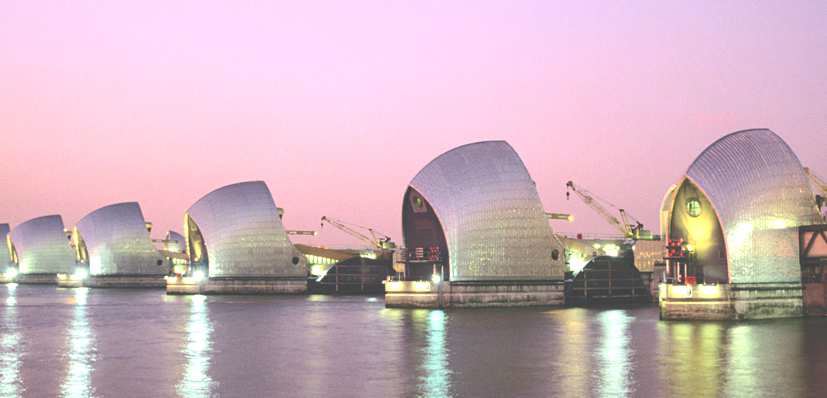
\includegraphics[width=\linewidth]{fig_00}
\end{marginfigure}


\subsection*{Contexte}

Pensé pour minimiser le temps de formation pour le patient et le thérapeute, l’exosquelette Atalante (figure 1),
 développé par la société Wandercraft a pour volonté d’optimiser les séances de rééducation, et à terme d’aboutir  à une solution permettant l’autonomie quasi totale du patient. En effet, ce système permet la verticalisation et
 des déplacements pouvant s’affranchir de toute dépendance à une tierce personne. De par sa liberté d’utilisation
 pour le patient, les bénéfices sont importants : possibilité de retours sensoriels, flexibilité de l’entrainement à la
 marche et à la course ou encore personnalisation des programmes proposés.

Les hypothèses et notations seront les suivantes (figure \ref{\label{Cy_04_03_PFD_CO_TD_01_fig_04}}) :
\begin{itemize}
  \item l'étude est menée dans le plan sagittal $\left(A, \vec{y}_{1}, \vec{z}_{1}\right)$, où $\vec{z}_{1}$ est vertical ascendant ;
  \item les différentes caractéristiques de dimension, masse et inertie des différents solides sont précisées annexe B ;
  \item le buste 1 étant animé d'un mouvement de translation rectiligne uniforme par rapport au référentiel terrestre, il est considéré comme galiléen ;
  \item l'étude se limite à la partie de la marche pour laquelle une des deux jambes est totalement décollée du sol (de $70 \%$ à $100 \%$ de la foulée);% sur la figure 3) ;
  \item le buste 1 est en liaison pivot d'axe $\left(A, \vec{x}_{1}\right)$ avec la cuisse 2 ; on note $\theta_{1}=\left(\vec{y}_{1}, \vec{y}_{2}\right)=\left(\vec{z}_{1}, \vec{z}_{2}\right)$;
  \item l'ensemble \{pied+tibia 3 , considéré comme solidaire, est en liaison pivot d'axe $\left(B, \vec{x}_{1}\right)$ avec la cuisse 2 ; on note $\theta_{2}=\left(\vec{y}_{2}, \vec{y}_{3}\right)=\left(\vec{z}_{2}, \vec{z}_{3}\right)$;
  \item les liaisons décrites précédemment sont supposées parfaites.
\end{itemize}

\begin{figure}
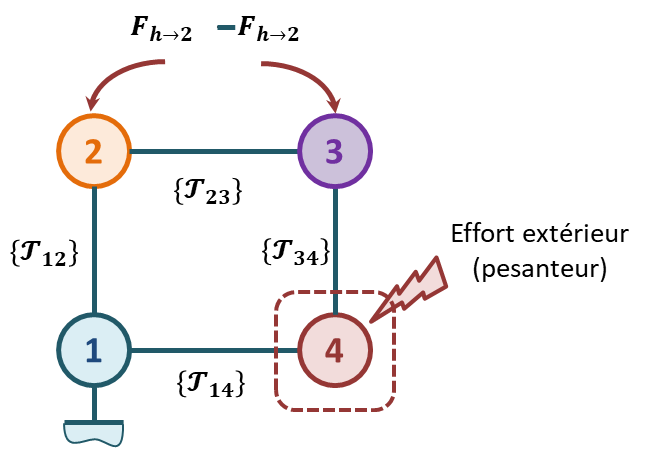
\includegraphics[max width=\textwidth, center]{fig_04}
\caption{Modélisation utilisée pour la marche en ligne droite \label{Cy_04_03_PFD_CO_TD_01_fig_04}}
\end{figure}

%\section{II Élaboration et analyse d'un modèle dynamique de l'exosquelette}
\begin{obj}
Définir un modèle dynamique de l’exosquelette et montrer la nécessité de mettre en place un asservissement.
\end{obj}

Afin d'élaborer une commande pour l'exosquelette, il est nécessaire au préalable de définir un modèle dynamique représentatif de son comportement. Seule la commande des articulations sagittales de hanche et de genou d'une jambe lorsqu'elle est décollée du sol %(figure 7 et hypothèses associées) 
sera considérée ici (cas de la marche en ligne droite) avec les hypothèses et notations supplémentaires suivantes, en plus de celles énoncées à la partie précédente :

\begin{itemize}
  \item la liaison pivot entre 1 et 2 est équipée d'un actionneur dont le couple de sortie (appliqué par 1 sur 2 ) est noté $C_{1}$;

  \item la liaison pivot entre 2 et 3 est équipée d'un actionneur dont le couple de sortie (appliqué par 2 sur 3 ) est noté $C_{2}$;

  \item les différentes caractéristiques géométriques, de masses et d'inerties sont données en annexe B ;

  \item on note respectivement $C_{\text {genou }}$ et $C_{\text {hanche }}$, les couples appliqués par le patient au niveau des articulations de genou et de hanche.

\end{itemize}

Le modèle dynamique proposé sera explicité pour mettre en évidence la nécessité d'un asservissement et par la suite (partie III), permettre l'élaboration de la loi de commande globale de l'exosquelette.

\section{II.A - Comportement dynamique de l'exosquelette}
On pose pour la suite : $\overrightarrow{B G_{3}}=-L_{0} \vec{z}^{\prime}$. On note $\alpha$ l'angle entre $\vec{z}^{\prime}{ }_{3}$ et $\vec{z}_{3}: \alpha=\left(\vec{y}_{3}, \vec{y}^{\prime}{ }_{3}\right)=\left(\vec{z}_{3}, \vec{z}^{\prime}{ }_{3}\right)$.

Q 6. Déterminer les expressions de $L_{0}$ et $\alpha$ en fonction de $l_{0}, L_{3}$ et $l_{3}$, puis calculer leurs valeurs numériques.

Q 7. Déterminer l'expression de l'accélération du point $G_{3}$ (cf. annexe B et question 6) appartenant à l'ensemble \{pied+tibia\} 3 dans son mouvement par rapport au buste 1 , en fonction de $L_{0}, L_{2}, \theta_{1}, \theta_{2}$ et leurs dérivées temporelles.

Q 8. Déterminer l'expression de la projection suivant $\vec{x}_{1}$ du moment dynamique en $A$ de l'ensemble $\{$ pied+tibia $\}$ 3 dans son mouvement par rapport au buste $1, \vec{\delta}_{A, 3 / 1} \cdot \vec{x}_{1}$, sous la forme :

$$
\vec{\delta}_{A, 3 / 1} \cdot \vec{x}_{1}=A_{1} \ddot{\theta}_{1}+A_{2} \ddot{\theta}_{2}+A_{3} \dot{\theta}_{1}^{2}+A_{4}\left(\dot{\theta}_{1}+\dot{\theta}_{2}\right)^{2}
$$

Préciser les expressions littérales de $A_{1}, A_{2}, A_{3}$ et $A_{4}$ en fonction des différentes caractéristiques géométriques, de masses et d'inerties de l'exosquelette.

Q 9. Proposer une démarche permettant de déterminer l'expression de $C_{1}$, l'action mécanique exercée sur la cuisse 2 par l'actionneur correspondant. Préciser le(les) ensemble(s) isolé(s), le(s) bilan(s) des actions mécaniques extérieurs, le(s) théorème(s) utilisé(s) et la(les) équation(s) utile(s).

Q 10. Déterminer l'expression de $C_{1}$ en fonction de $\theta_{1}, \theta_{2}$, leurs différentes dérivées, de $C_{\text {hanche }}$ et des différentes caractéristiques géométriques, de masses et d'inerties de l'exosquelette.

D'une manière similaire aux questions précédentes, l'application du principe fondamental de la dynamique à l'ensemble \{pied+tibia\} 3 permet d'obtenir l'expression de $C_{2}$, le couple fourni par l'actionneur de genou sagittal :

$$
C_{2}=\left[I_{x 3}+m_{3} L_{0}^{2}\right]\left(\ddot{\theta}_{1}+\ddot{\theta}_{2}\right)+m_{3} L_{2} L_{0}\left[\ddot{\theta}_{1} \cos \left(\theta_{2}+\alpha\right)+\dot{\theta}_{1}^{2} \sin \left(\theta_{2}+\alpha\right)\right]+m_{3} g L_{0} \sin \left(\theta_{2}+\theta_{1}+\alpha\right)-C_{\text {genou }}
$$

Q 11. Déduire des deux équations précédentes que le modèle dynamique considéré peut s'écrire sous la forme matricielle suivante :

$$
\left(\begin{array}{l}
C_{1} \\
C_{2}
\end{array}\right)=M_{1}\left(\begin{array}{c}
\ddot{\theta}_{1} \\
\ddot{\theta}_{2}
\end{array}\right)+M_{2}\left(\begin{array}{c}
\dot{\theta}_{1} \\
\dot{\theta}_{2}
\end{array}\right)+C+M_{3}\left(\begin{array}{c}
C_{\text {hanche }} \\
C_{\text {genou }}
\end{array}\right)
$$

où $C$ est une matrice colonne et $M_{1}, M_{2}$ et $M_{3}$ sont des matrices $2 \times 2$. Donner l'expression littérale des coefficients de $C, M_{1}, M_{2}$ et $M_{3}$ par des relations non linéaires des paramètres de mouvement $\left(\theta_{1}, \theta_{2}\right)$, leurs dérivés premières et des différentes caractéristiques géométriques, de masses et d'inerties du problème.
